\documentclass[a4paper,14pt]{extarticle}

\usepackage{fontspec}
\usepackage{polyglossia}
\setdefaultlanguage{russian}
\setotherlanguage{english}
\setmainfont{Times New Roman}
\setmonofont{PT Mono}

\usepackage{geometry}
\geometry{left=30mm, right=10mm, top=20mm, bottom=20mm}

\usepackage{amsmath}
\usepackage{xcolor}
\usepackage{graphicx}
\usepackage{setspace}
\usepackage[normalem]{ulem}
\usepackage{float}
\usepackage{caption}
\usepackage{listings}
\usepackage[hidelinks]{hyperref}

\usepackage{bmstu-title}

% --- данные титульного листа -------------------------------------------------
\newcommand{\workfaculty}{Информатика и системы управления}
\newcommand{\workchair}{Программное обеспечение ЭВМ и информационные технологии (ИУ7)}
\newcommand{\workkind}{лабораторной работе №~1\\}
\newcommand{\workcourse}{Операционные системы}
\newcommand{\workstudent}{Д.~С.~Дудырев}
\newcommand{\workgroup}{ИУ7-52Б}
\newcommand{\workteacher}{Н.~Ю.~Рязанова}
% -----------------------------------------------------------------------------

\captionsetup[figure]{name=Рисунок, labelsep=endash, justification=centering}
\renewcommand{\lstlistingname}{Листинг}
\captionsetup[lstlisting]{labelsep=endash, singlelinecheck=false, skip=4pt}

\lstset{
    basicstyle   = \ttfamily\fontsize{7.6}{8.7}\selectfont,
    columns      = fullflexible,
    keepspaces   = true,
    breaklines   = true,
    breakindent  = 0pt,
    breakautoindent = false,
    frame        = single,
    framesep     = 4pt,
    rulecolor    = \color{black},
    captionpos   = t,
    numbers      = none,
    showstringspaces = false,
}

\onehalfspacing
\setlength{\parindent}{1.25cm}

\begin{document}

\makereporttitle
    {\workfaculty}
    {\workchair}
    {\workkind}
    {\workcourse}
    {}
    {}
    {\workstudent/\workgroup}
    {\workteacher}

\begin{center}
    \large\bfseries Дизассемблированный код
\end{center}
\vspace{3mm}

\lstinputlisting[caption={Обработчик прерывания INT 8h}]{listing-int08.lst}

\clearpage

\lstinputlisting[caption={Подпрограмма sub\_1}]{listing-sub1.lst}

\clearpage

\begin{center}
    \large\bfseries Схемы алгоритмов
\end{center}
\vspace{5mm}

\begin{figure}[H]
    \centering
    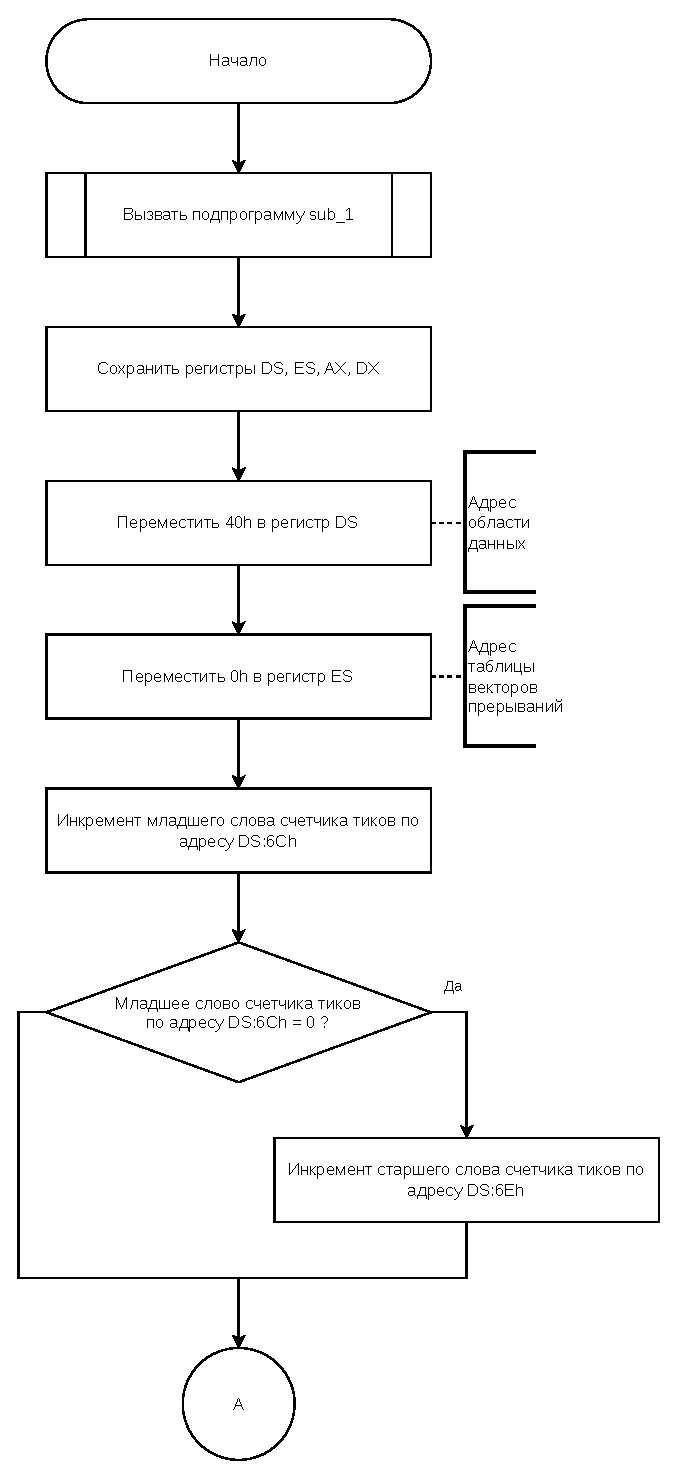
\includegraphics[page=1, width=\textwidth, height=0.82\textheight, keepaspectratio]{algo-crop.pdf}
    \caption{Схема алгоритма работы обработчика прерывания INT 8h}
\end{figure}

\clearpage

\begin{figure}[H]
    \centering
    \includegraphics[page=2, width=\textwidth, height=0.82\textheight, keepaspectratio]{algo-crop.pdf}
    \caption{Схема алгоритма работы обработчика прерывания INT 8h}
\end{figure}

\clearpage

\begin{figure}[H]
    \centering
    \includegraphics[page=3, width=\textwidth, height=0.82\textheight, keepaspectratio]{algo-crop.pdf}
    \caption{Схема алгоритма работы обработчика прерывания INT 8h}
\end{figure}

\clearpage

\begin{figure}[H]
    \centering
    \includegraphics[page=4, width=\textwidth, height=0.82\textheight, keepaspectratio]{algo-crop.pdf}
    \caption{Схема алгоритма работы обработчика прерывания INT 8h}
\end{figure}

\clearpage

\begin{figure}[H]
    \centering
    \includegraphics[page=5, width=\textwidth, height=0.82\textheight, keepaspectratio]{algo-crop.pdf}
    \caption{Схема алгоритма работы подпрограммы sub\_1}
\end{figure}

\end{document}
